	
\subsubsection{29.09.14}

\begin{enumerate}
	\item Время начала и окончания собрания:
	18:00 - 21:30
	\item Цели собрания:
	\begin{enumerate}
	  \item Обсудить правила FTC.
	  
	  \item Разобрать основные аспекты конструкции робота.
	  
      \item Разработать стратегию игры нашей команды.
    \end{enumerate}
	\item Проделанная работа:
	\begin{enumerate}
	  \item Была обсуждена 2 часть правил, с которыми каждый из нас предварительно ознакомился самостоятельно.
	  
	  \item В ходе обсуждения конструкции робота было выдвинуто несколько идей:
	  \begin{enumerate}
	    \item Размеры робота:
	    \begin{enumerate}
	      \item Робот должен быто достаточно компактным, чтобы помимо самого корпуса в размеры помещался еще и захват для мячей.
	      
	      \item Робот должен быть компактным, чтобы не мешать союзникам.
	      
	      \item Корпус робота не должен быть слишком маленьким, иначе он будет неустойчив в разложенном состоянии с вытянутым ковшом (максимальная высота поднятия – 120 см).
	      
	    \end{enumerate}
	    
	    \item Колесная база:
	    \begin{enumerate}
	      \item Конструкция с четырьмя ведущими колесами, центры которых находятся в углах квадрата. Такая система также хорошо ездит по прямой и разворачивается на месте, но в отличие от предыдущей занимает значительно меньше места и практически неразрушаема, что имеет важную роль в соревнованиях FTC. Незначительным минусом конструкции является то, что при развороте колеса неспособны катиться и подпрыгивают, из-за чего робот ощутимо трясется.	
	      
	      \item Конструкция с двумя гусеницами. Плюсы данной конструкции заключаются в том, что она отлично ездит по прямой  и разворачивается на месте вокруг точки пересечения диагоналей прямоугольника, в углах которого располагаются катки. Минусами системы являются большие размеры и ненадежность, поскольку гусеница может слететь в самый ответственный момент. Кроме того, в нашем наборе TETRIX отсутствуют гусеницы, поэтому в случае выбора данной конструкции их предстоит сделать самостоятельно.
	      
	      \item Конструкция с четырьмя ведущими омни-колесами из набора TETRIX, центры которых находятся в углах квадрата, расположенными под углом в 45 градусов к корпусу. Превосходство данной конструкции над предыдущими в том, что она способна двигаться не только вперед или назад, а во всех направлениях. Эта конструкция позволяет роботу очень быстро поворачиваться на месте, но плохо показывает себя при движении по прямой, что может негативно сказаться на автономном периоде.
	      
	      \item Конструкция с четырьмя ведущими омни-колесами, в которых ролики располагаются под углом в 45 градусов к направлению вращения колеса, центры которых находятся в углах квадрата, таким же образом, как в случае с обычными колесами. Плюсы: точное движение по прямой, быстрый разворот на месте, возможность движения в любом направлении без поворота корпуса. Минусы: необходимость докупать колеса отдельно в связи с отсутствием таковых в наборе, низкая точность при развороте.
	      
	      \begin{figure}[h]
	      	\begin{minipage}[h]{0.165\linewidth}
	      		\center  
	      	\end{minipage}
	      	\begin{minipage}[h]{0.6\linewidth}
	          \center{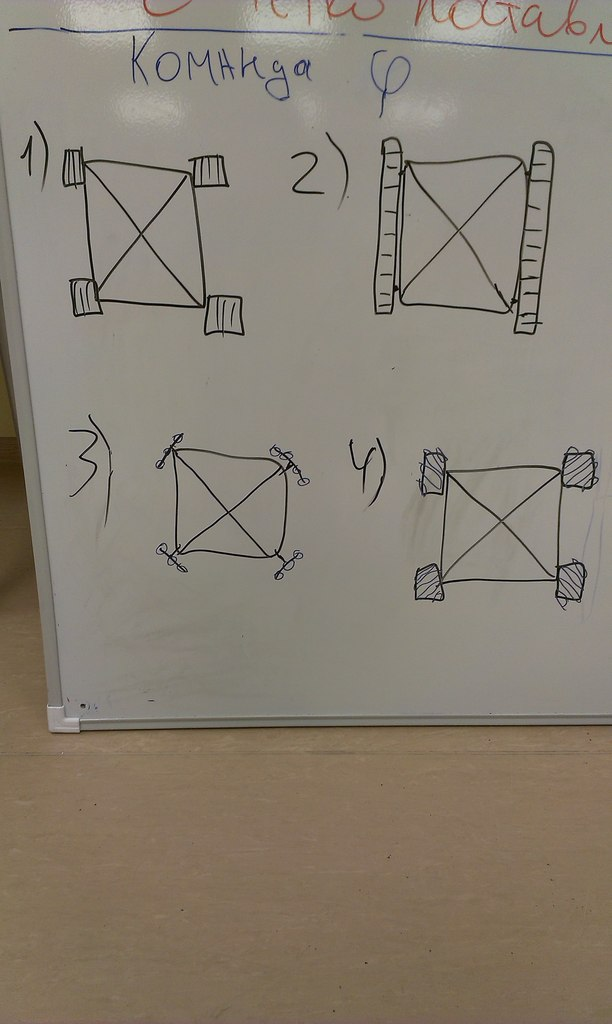
\includegraphics[scale=0.3]{days/29.09.14/images/01}}
	          \caption{Идеи для ходовой: 1)Конструкция с четырьмя ведущими колесами 2)Конструкция с двумя гусеницами 3) Конструкция с четырьмя ведущими омни-колесами из набора TETRIX 4)Конструкция с четырьмя ведущими омни-колесами}
	        \end{minipage}
	      \end{figure}
	      
	    \end{enumerate}
	    
	    \item Система контроля мячей:
	    \begin{enumerate}
	      \item Корзина для шаров закреплена на системе из некоторого количества реек, соединенных между собой сервоприводами. Плюсы: отсутствие лески, способной порваться в ходе соревнований. Минусы: чрезмерная сложность и громоздкость конструкции вкупе с ее слабой надежностью.	
	      
	      \item Корзина для шаров закреплена на вертикальных раздвижных мебельных рейках, основание которых жестко зафиксировано на каркасе робота, а механизм раздвигания приводится в действие DC-мотором, наматывающим на себя леску. Плюсы: простота и надежность конструкции (за исключением лески), высокая точность подъема корзины-захвата на заданную высоту. Минусы: леска способна порваться в ходе соревнований
	      
	      \item Корзина для шаров закреплена на раздвижных мебельных рейках, механизм раздвигания которых приводится в действие DC-мотором, наматывающим на себя леску, а основание установлено на оси другого DC-мотора, способного поворачивать ее в вертикальной плоскости, параллельной длине робота. Плюсы: возможность раздвигания системы в горизонтальном положении снимает часть нагрузки с лески, точность подъема корзины-захвата на заданную высоту средняя. Минусы: леска способна порваться в ходе соревнований.
	      
	      \begin{figure}[H]
	      	\begin{minipage}[h]{0.2\linewidth}
	      		\center  
	      	\end{minipage}
	      	\begin{minipage}[h]{0.6\linewidth}
	      		\center{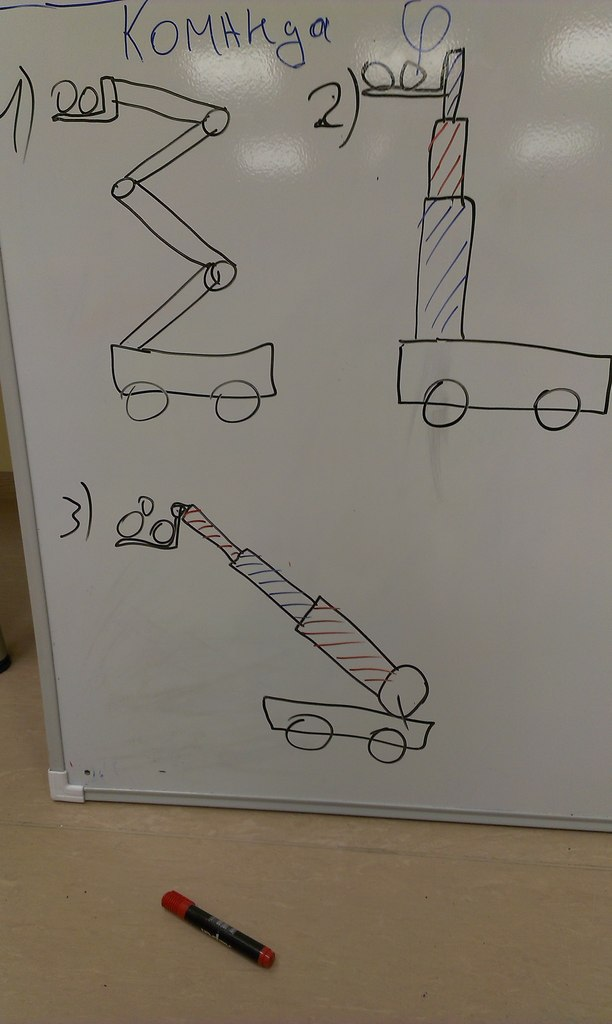
\includegraphics[scale=0.3]{days/29.09.14/images/02}}
	      		\caption{Идеи для подъемника мячей: 1)Конструкция №1 б)Конструкция с неподвижными мебельными рейками в) Конструкция с мебельными рейками, установленными на вращающейся платформе}
	      	\end{minipage}
	      \end{figure}
	      
	    \end{enumerate}
	    
	    \item Система фиксирования подвижной корзины (для более точного закидывания мячей в корзину, а также для транспортировки ее в зону парковки):
	    \begin{enumerate}
	      \item П-образный захват с двумя сервоприводами, фиксирующими корзину между балками, установленный на оси DC-мотора, способного поворачивать ее в вертикальной плоскости, параллельной длине робота. Плюсы: способность поднимать корзины над полом, входит в размеры в сложенном состоянии. Минусы: занимает много места.
	      
          \item Такой же захват, только вместо балок-клешней используются крючки, способные захватывать корзину за отверстия, расположенные в ее основании. Плюсы: компактнее предыдущего варианта. Минусы: Попадать крючками в отверстия будет довольно трудно.
          
			\begin{figure}[H]
				\begin{minipage}[h]{0.2\linewidth}
					\center  
				\end{minipage}
				\begin{minipage}[h]{0.6\linewidth}
					\center{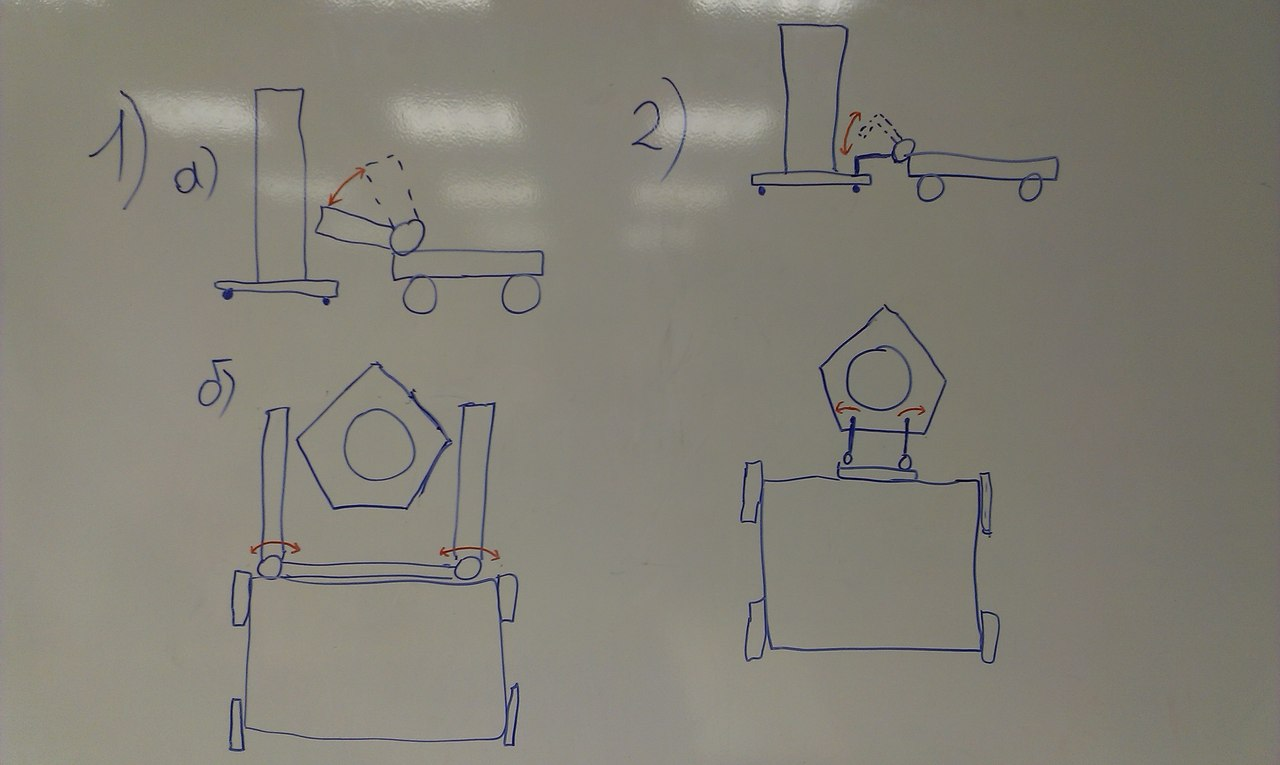
\includegraphics[scale=0.25]{days/29.09.14/images/03}}
          		\caption{Идеи фиксирования подвижной корзины: 1)П-образный захват 2)Захват с крючками}
				\end{minipage}
			\end{figure}
          
        \end{enumerate}
      \end{enumerate}
    \end{enumerate}
    
	\item Итоги собрания: 
	\begin{enumerate}
	  \item В результате обсуждения были сформированы общие идеи, касающиеся нашего проекта. Они были помещены в разделы «Концепция робота»,  «Стратегия» и «Планируемые этапы создания робота».
	  
      \item Было определено общее направление приложения усилий, однако ничего конкретного пока решено не было.
      
    \end{enumerate}
    
	\item Задачи для последующих собраний:
	\begin{enumerate}
	  \item Выбрать оптимальную колесную базу.
	  
	  \item Выбрать оптимальный размер корпуса робота, исходя из соображений компактности и устойчивости.
	  
	  \item Выбрать наилучшую систему контроля шаров.
	  
	  \item Выбрать наиболее эффективный вид фиксирования подвижной корзины.
	  
    \end{enumerate}
\end{enumerate}
\fillpage


